\documentclass{article}
\usepackage[preprint]{neurips_2026}

\usepackage[utf8]{inputenc}
\usepackage[T1]{fontenc}
\usepackage{hyperref}
\usepackage{url}
\usepackage{booktabs}
\usepackage{amsfonts}
\usepackage{amsmath}
\usepackage{amssymb}
\usepackage{nicefrac}
\usepackage{microtype}
\usepackage{xcolor}
\usepackage{graphicx}
\usepackage{subcaption}
\usepackage{float}
\usepackage{booktabs}

\workshoptitle{WORKSHOP TITLE}

\title{Assignment for \emph{``Advanced Statistical Inference'' 2026}\\
Auto-Encoding Variational Bayes}

\author{%
  Author \\
  \texttt{email} \\
  \And
  Author \\
  \texttt{email} \\
}

\begin{document}
\maketitle

\begin{abstract}
Abstract here
\end{abstract}3

%%%%%%%%%%%%%%%%%%%%%%%%%%%%%%%%%%%%%%%%%%%%%%%%%%%%%%%%%%%%
\section{Paper Summary}
%%%%%%%%%%%%%%%%%%%%%%%%%%%%%%%%%%%%%%%%%%%%%%%%%%%%%%%%%%%%

\subsection{The Central Problem}

A recurring challenge in Bayesian inference is the computation of the posterior
distribution $p(\mathbf{z} \mid \mathbf{x})$, which describes the distribution
over latent variables $\mathbf{z}$ given an observation $\mathbf{x}$.
By Bayes' rule:
\[
  p(\mathbf{z} \mid \mathbf{x}) = \frac{p(\mathbf{x} \mid \mathbf{z})\, p(\mathbf{z})}{p(\mathbf{x})},
\]
where $p(\mathbf{x}) = \int p(\mathbf{x} \mid \mathbf{z})\, p(\mathbf{z})\, d\mathbf{z}$
is the marginal likelihood (or \emph{evidence}).
This integral is intractable for most models of practical interest, as it requires
integrating over the entire latent space.
Classical alternatives each carry significant trade-offs: MCMC methods are asymptotically
exact but computationally expensive; the Laplace approximation is fast but restricted
to locally Gaussian posteriors; mean-field variational inference requires analytical
expectations that are themselves often intractable.

\subsection{Variational Inference and the ELBO}

Kingma and Welling~\cite{kingma2013} address this by directly approximating the true
posterior with a simpler, parametric distribution $q_{\boldsymbol{\phi}}(\mathbf{z} \mid \mathbf{x})$
--- a multivariate Gaussian with diagonal covariance.
The goal is to make $q_{\boldsymbol{\phi}}$ as close as possible to the true posterior
$p_{\boldsymbol{\theta}}(\mathbf{z} \mid \mathbf{x})$, where closeness is measured by
the KL divergence $D_{\mathrm{KL}}(q_{\boldsymbol{\phi}} \| p_{\boldsymbol{\theta}})$.

The key algebraic insight comes from decomposing the log marginal likelihood:
\[
  \log p_{\boldsymbol{\theta}}(\mathbf{x})
  = \mathcal{L}(\boldsymbol{\theta}, \boldsymbol{\phi};\, \mathbf{x})
  + D_{\mathrm{KL}}\!\left(q_{\boldsymbol{\phi}}(\mathbf{z} \mid \mathbf{x})
    \;\|\; p_{\boldsymbol{\theta}}(\mathbf{z} \mid \mathbf{x})\right),
\]
where $\mathcal{L}(\boldsymbol{\theta}, \boldsymbol{\phi};\, \mathbf{x})$ is the
\emph{Evidence Lower BOund} (ELBO). Since the log evidence is fixed with respect to
$\boldsymbol{\phi}$ and the KL divergence is non-negative, maximizing the ELBO is
equivalent to minimizing the KL divergence --- without ever computing $p(\mathbf{x})$.

The ELBO itself decomposes into two interpretable terms:
\[
  \mathcal{L}(\boldsymbol{\theta}, \boldsymbol{\phi};\, \mathbf{x})
  = \underbrace{-D_{\mathrm{KL}}\!\left(q_{\boldsymbol{\phi}}(\mathbf{z} \mid \mathbf{x})
    \;\|\; p_{\boldsymbol{\theta}}(\mathbf{z})\right)}_{\text{regularization}}
  + \underbrace{\mathbb{E}_{q_{\boldsymbol{\phi}}(\mathbf{z} \mid \mathbf{x})}
    \!\left[\log p_{\boldsymbol{\theta}}(\mathbf{x} \mid \mathbf{z})\right]}_{\text{reconstruction}}.
\]
When both the prior $p_{\boldsymbol{\theta}}(\mathbf{z}) = \mathcal{N}(\mathbf{0}, \mathbf{I})$
and the approximate posterior $q_{\boldsymbol{\phi}}(\mathbf{z} \mid \mathbf{x})$ are
Gaussian, the KL term has a closed-form solution (Appendix~B of the paper).
The reconstruction term is estimated by Monte Carlo with $L=1$ sample per datapoint,
which the authors show to be sufficient when the minibatch size $M$ is large enough.

\subsection{The Reparameterization Trick}

A naive Monte Carlo gradient estimator for the ELBO fails because sampling
$\mathbf{z} \sim q_{\boldsymbol{\phi}}(\mathbf{z} \mid \mathbf{x})$
introduces a discontinuity with respect to $\boldsymbol{\phi}$, yielding
a gradient estimator of prohibitively high variance.
The paper resolves this with the \emph{reparameterization trick}: instead of
sampling $\mathbf{z}$ directly, one writes
\[
  \mathbf{z} = \boldsymbol{\mu}_{\boldsymbol{\phi}}(\mathbf{x})
             + \boldsymbol{\sigma}_{\boldsymbol{\phi}}(\mathbf{x}) \odot \boldsymbol{\varepsilon},
  \qquad \boldsymbol{\varepsilon} \sim \mathcal{N}(\mathbf{0}, \mathbf{I}).
\]
The stochasticity is now in $\boldsymbol{\varepsilon}$, which is independent of
$\boldsymbol{\phi}$, so the gradient $\nabla_{\boldsymbol{\phi}} \mathcal{L}$ can
be computed by standard backpropagation.
This yields the Stochastic Gradient Variational Bayes (SGVB) estimator, which
is then optimized over minibatches of size $M = 100$ using Adagrad.

\subsection{The Variational Autoencoder}

As a concrete instantiation, the authors parameterize both the approximate posterior
and the generative model with multi-layer perceptrons, giving rise to the
\emph{Variational Autoencoder} (VAE).

The \textbf{encoder} network $q_{\boldsymbol{\phi}}(\mathbf{z} \mid \mathbf{x})$
takes an observation $\mathbf{x}$ as input and outputs the mean
$\boldsymbol{\mu}$ and log-variance $\log \boldsymbol{\sigma}^2$ of the
approximate posterior Gaussian. It provides an efficient, amortized inference
mechanism: rather than optimizing variational parameters per datapoint, a single
network generalizes across the dataset.

The \textbf{decoder} network $p_{\boldsymbol{\theta}}(\mathbf{x} \mid \mathbf{z})$
takes a latent sample $\mathbf{z}$ and reconstructs the observation --- using a
Bernoulli MLP for binary data (MNIST) or a Gaussian MLP for continuous data
(Frey Face).

Both networks are trained jointly by maximizing the ELBO: the decoder learns to
reconstruct faithfully, while the KL term regularizes the encoder to produce a
latent space close to the isotropic Gaussian prior.
This structured latent space enables three practical capabilities beyond standard
autoencoders: (1) \emph{generation} of new samples by drawing $\mathbf{z} \sim \mathcal{N}(\mathbf{0}, \mathbf{I})$
and decoding; (2) \emph{smooth interpolation} between observations in latent space;
and (3) \emph{compact representation learning} for downstream tasks such as
classification or retrieval. Without the KL regularization term, the latent space
would be unstructured and sampling from it would yield incoherent outputs.

%%%%%%%%%%%%%%%%%%%%%%%%%%%%%%%%%%%%%%%%%%%%%%%%%%%%%%%%%%%%
\section{Reproduced Results}
%%%%%%%%%%%%%%%%%%%%%%%%%%%%%%%%%%%%%%%%%%%%%%%%%%%%%%%%%%%%

We reproduced the three main experiments reported in the paper: (1) the evolution of
the variational lower bound (ELBO) during training for varying latent dimensionalities
$N_z$, on both MNIST and Frey Face; (2) the visualization of the learned 2-D latent
manifold; and (3) random samples from the generative model for different values of $N_z$.

\paragraph{Implementation.}
The encoder and decoder follow the architecture specified in Appendix~C of the
paper~\cite{kingma2013}: single hidden layer MLPs with $\tanh$ activations, 500
hidden units for MNIST and 200 for Frey Face. The decoder uses a Bernoulli MLP for
MNIST (binary cross-entropy reconstruction loss) and a Gaussian MLP for Frey Face
(mean squared error with learned variance). The prior is $p(\mathbf{z}) =
\mathcal{N}(\mathbf{0}, \mathbf{I})$, the KL term is computed analytically, and
$L=1$ Monte Carlo sample is drawn per datapoint. Optimization uses Adagrad with
learning rate $0.01$ and weight decay $10^{-4}$, matching the MAP criterion described
in the paper. The minibatch size is $M=500$ rather than the paper's $M=100$, a choice
motivated by the GPU-oriented training environment on Kaggle.
Models were trained for 200~epochs on MNIST (60\,000 training samples) and on
a subset of 1\,500 samples for Frey Face, with the remaining 465 samples used as
a test set. Experiments were run for $N_z \in \{2, 5, 10, 20\}$; the paper additionally
reports $N_z = 200$ for MNIST, which was omitted here due to computational constraints.
The full implementation is available as a Jupyter notebook in the accompanying
repository.

\paragraph{ELBO during training (Figure~\ref{fig:elbo}).}
Figure~\ref{fig:elbo} reproduces Figure~2 of the paper. The horizontal axis shows the
training epoch rather than the number of training samples evaluated (as in the paper,
where a logarithmic scale is used); 200~epochs on MNIST correspond to approximately
$1.2 \times 10^7$ sample evaluations, which covers the same effective training budget.
On MNIST, the ELBO improves monotonically with $N_z$ and the train/test curves
track closely throughout training, confirming the regularizing effect of the KL term
noted by the authors. The final test ELBO values are reported in
Table~\ref{tab:elbo_mnist} alongside the approximate values read from the paper.
For $N_z = 20$, our model reaches $-93$, which is slightly above the paper's $-100$;
this gap is likely attributable to the larger minibatch size ($M=500$), which reduces
gradient variance and accelerates convergence.
For $N_z = 5$, convergence is slower and the final value ($-118$) remains below the
paper's $-103$, suggesting that 200~epochs may not be sufficient for smaller latent
spaces.

On Frey Face, the qualitative behavior matches the paper: the ELBO increases rapidly
in the first 50 epochs and continues to improve slowly thereafter, with no sign of
overfitting. However, the test curve exhibits high variance (visible as noise around
the smooth trend in Figure~\ref{fig:elbo_ff}), unlike the smooth test curve in the
paper. This is a direct consequence of the small test set (465~samples): with $L=1$
and a single evaluation pass, the Monte Carlo estimate of the ELBO has high variance
per epoch. The paper likely used a larger or differently split test set. Final test
ELBO values on Frey Face are approximately $1\,200$, $1\,250$, $1\,550$, and
$1\,550$ for $N_z = 2, 5, 10, 20$ respectively, compared to~$\approx 1\,600$ in
the paper for all $N_z$.

\paragraph{Comparison with Wake-Sleep.}
Following the paper's Figure~2, we also trained a Wake-Sleep model with identical
architectures and hyperparameters for each $N_z$ and dataset, and overlay its ELBO
curves (green) on the AEVB curves (red) in Figures~\ref{fig:elbo} and~\ref{fig:elbo_ff}.

On MNIST, the advantage of AEVB is clear across all latent dimensions. AEVB converges
rapidly within the first 50--80 epochs, whereas the Wake-Sleep curves are still
visibly increasing at epoch 200 --- convergence was not reached within the available
training budget. The gap in final test ELBO is substantial: approximately 42~points
for $N_z=2$ ($-150$ vs $-192$), 37 for $N_z=5$ ($-120$ vs $-157$), 41 for $N_z=10$
($-100$ vs $-141$), and 54 for $N_z=20$ ($-93$ vs $-147$). These figures are consistent
with the advantage reported in the paper.

On Frey Face, the same pattern holds: AEVB curves consistently sit above Wake-Sleep
for all $N_z$, though both exhibit high variance due to the small test set.
Wake-Sleep final test ELBO values are approximately $950$, $1\,100$, $1\,100$,
and $1\,150$ for $N_z = 2, 5, 10, 20$ respectively, compared to $1\,200$--$1\,330$
for AEVB.

Wake-Sleep training was significantly more expensive: each epoch requires two separate
optimization passes (a wake phase updating the decoder, and a sleep phase updating
the encoder), roughly doubling the per-epoch computation time relative to AEVB.
Running 200~epochs of Wake-Sleep for all eight models consumed a large fraction of
the available compute budget, and the models still had not converged --- confirming
that the ELBO gap is not merely an artifact of insufficient training time.

\begin{table}[H]
\centering
\caption{Final test ELBO on MNIST (per datapoint). Paper values are approximate,
read from Figure~2 of~\cite{kingma2013}. Our AEVB model uses $M=500$;
the paper uses $M=100$.}
\label{tab:elbo_mnist}
\begin{tabular}{lcccc}
\toprule
 & $N_z=2$ & $N_z=5$ & $N_z=10$ & $N_z=20$ \\
\midrule
Paper (approx.) & --- & $-103$ & $-101$ & $-100$ \\
AEVB (ours)     & $-150$ & $-118$ & $-100$ & $-93$ \\
Wake-Sleep (ours) & $-192$ & $-157$ & $-141$ & $-147$ \\
\bottomrule
\end{tabular}
\end{table}

\begin{figure}[H]
  \centering
  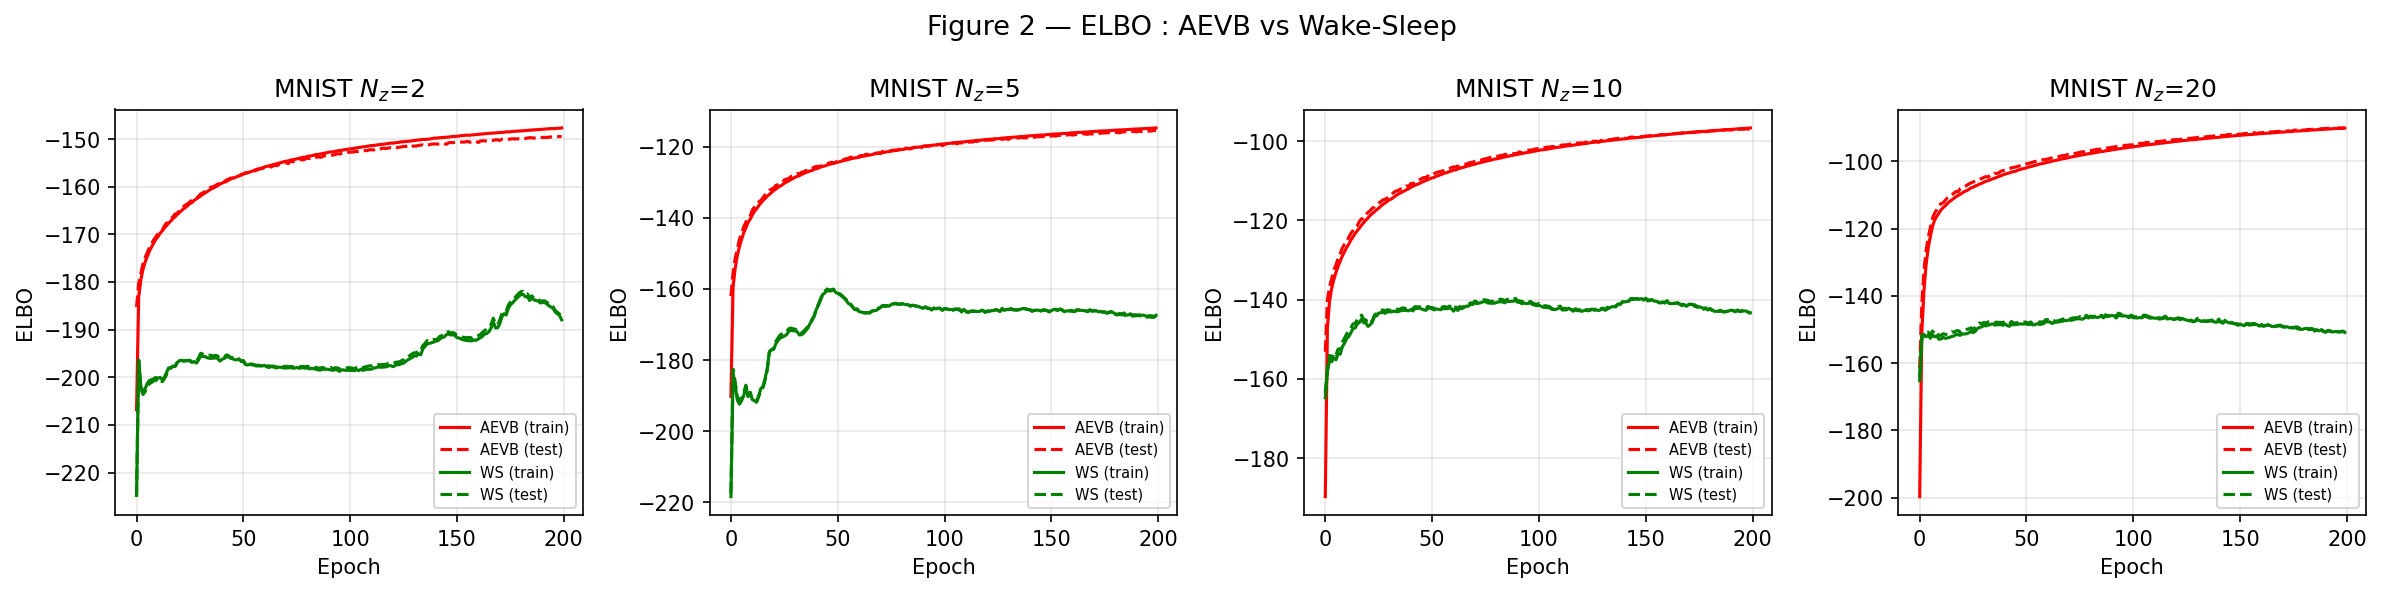
\includegraphics[width=\linewidth]{src/fig2_elbo_mnist.png}
  \caption{ELBO during training on MNIST for $N_z \in \{2, 5, 10, 20\}$.
  Red: AEVB (solid train, dashed test). Green: Wake-Sleep (solid train, dashed test).
  Wake-Sleep has not converged after 200~epochs and consistently falls 40--54~points
  below AEVB.}
  \label{fig:elbo}
\end{figure}

\begin{figure}[H]
  \centering
  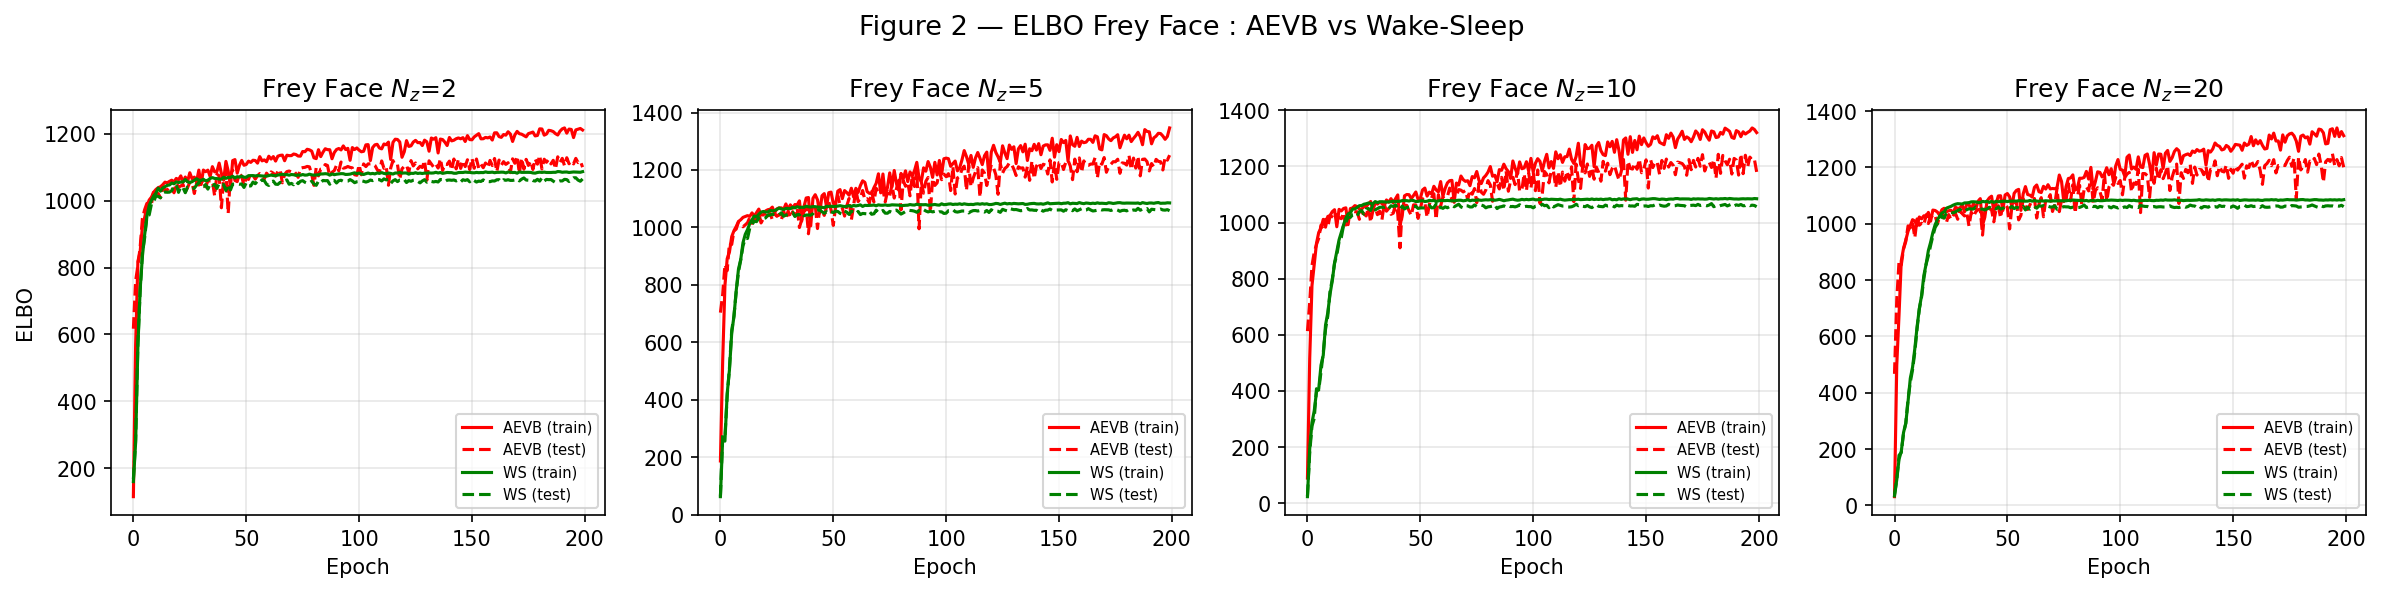
\includegraphics[width=\linewidth]{src/fig2_elbo_freyface.png}
  \caption{ELBO during training on Frey Face for $N_z \in \{2, 5, 10, 20\}$.
  Red: AEVB. Green: Wake-Sleep. Both exhibit high variance due to the small test
  set (465~samples, $L=1$); AEVB consistently reaches higher values.}
  \label{fig:elbo_ff}
\end{figure}

\paragraph{Random samples (Figure~\ref{fig:samples}).}
Figure~\ref{fig:samples} reproduces Figure~5 of the paper. Samples are drawn by
first sampling $\mathbf{z} \sim \mathcal{N}(\mathbf{0}, \mathbf{I})$ and decoding.
As in the paper, sample quality improves with $N_z$: digits become sharper and more
varied as the latent space grows. For small $N_z$, the decoder produces blurry,
superimposed-looking digits, consistent with the model averaging over multiple modes.

\begin{figure}[H]
  \centering
  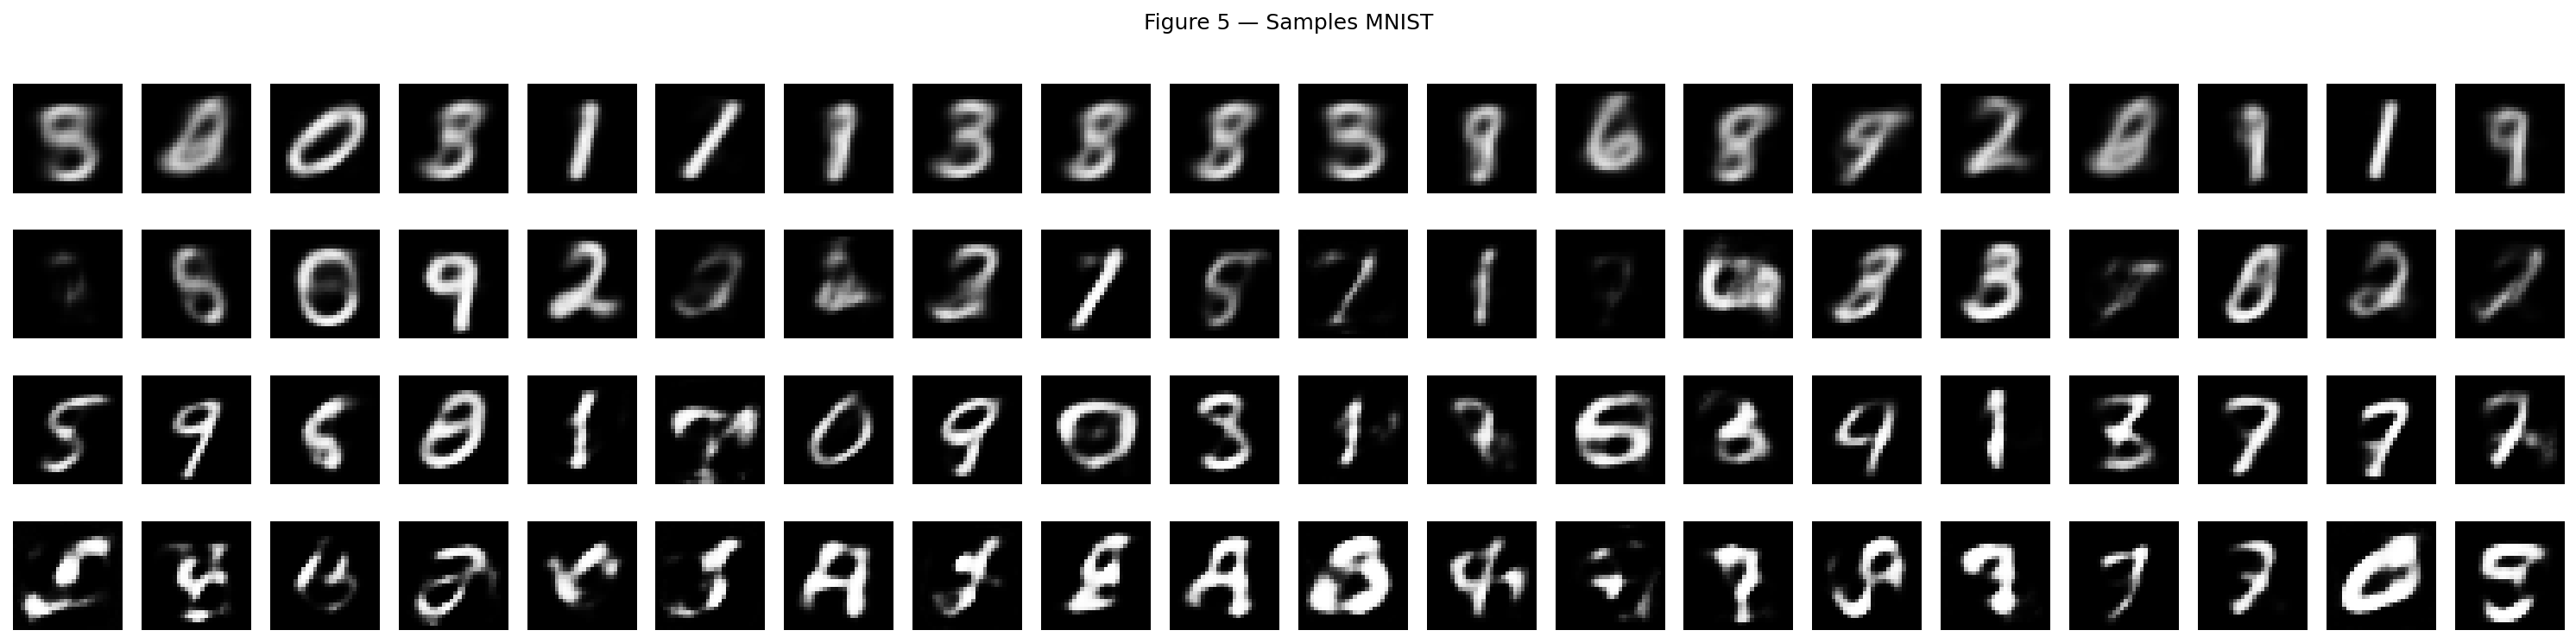
\includegraphics[width=0.75\linewidth]{src/fig5_samples.png}
  \caption{Random samples from the MNIST generative model for $N_z \in \{2,5,10,20\}$
  (rows, top to bottom).}
  \label{fig:samples}
\end{figure}

%%%%%%%%%%%%%%%%%%%%%%%%%%%%%%%%%%%%%%%%%%%%%%%%%%%%%%%%%%%%
\section{Discussion}
%%%%%%%%%%%%%%%%%%%%%%%%%%%%%%%%%%%%%%%%%%%%%%%%%%%%%%%%%%%%

\subsection{Conceptual Difficulty: Connecting $\boldsymbol{\phi}$ to Network Weights}
One recurring difficulty in understanding this paper is the gap between the
mathematical notation and its practical instantiation. The symbol $\boldsymbol{\phi}$
denotes all encoder parameters collectively, but when the encoder is a multi-layer
perceptron with several weight matrices, it is not immediately clear how the gradient
$\nabla_{\boldsymbol{\phi}} \mathcal{L}$ propagates through each layer back to
$\boldsymbol{\mu}$ and $\boldsymbol{\sigma}$, and ultimately to each weight matrix.
Building this intuition required tracing a full forward and backward pass manually
through a two-layer, two-neuron network, which revealed that the reparameterization
trick simply makes $\mathbf{z}$ a deterministic node in the computation graph, after
which standard chain rule applies layer by layer. This connection between
the compact notation of the paper and the mechanics of backpropagation was the
most time-consuming conceptual step.

A second, related difficulty is that the paper assumes a solid prior familiarity
with variational inference, directed graphical models, and KL divergences.
Concepts such as the ELBO decomposition, the closed-form KL between two Gaussians,
or the notion of amortized inference are used without derivation or commentary.
Filling these gaps required frequent back-and-forth with course notes and external
references, which added substantially to the time required to \emph{understand}
the paper --- as opposed to merely implementing it.

\subsection{Practical Training Constraints}
Reproducing the experiments exposed several practical limitations. Training was
conducted on Kaggle, whose session-based execution model does not persist
model checkpoints by default, requiring careful manual saving. More significantly,
training at the largest latent dimensionality reported in the paper
($\dim(\mathbf{z}) = 200$) was impractical: at that scale, a full 200-epoch run
would have been very long and would have consumed most or all of the available
compute quota. Results were therefore obtained at reduced scale ($N_z \leq 20$),
which limits direct comparison with the reported marginal log-likelihood values.

The Wake-Sleep comparison further illustrated this constraint. Because each epoch
requires two separate optimization phases, Wake-Sleep training took roughly twice
as long per epoch as AEVB. Running 200~epochs for all eight Wake-Sleep models
(4 values of $N_z$ $\times$ 2 datasets) consumed a large fraction of the available
compute budget --- and the models still had not converged by the end of training,
as visible in the ELBO curves of Figures~\ref{fig:elbo} and~\ref{fig:elbo_ff}.

\subsection{Unjustified Hyperparameter Choices}
Some design choices in the paper are presented without theoretical justification.
In particular, the minibatch size $M = 100$ is stated in Section~3 as sufficient
for the $L = 1$ Monte Carlo estimator to work well, but no ablation or sensitivity
analysis is provided. The choice appears empirical, and it is unclear how
performance degrades for smaller $M$ or different dataset statistics.

More generally, not all hyperparameters are fully specified: the number of training
epochs and the learning rate schedule, for instance, are not justified. A systematic
grid search over these choices would be needed to fairly reproduce the reported
results, but the compute quota constraints described above make exhaustive
experimentation impractical. This means that some of the paper's performance numbers
are difficult to reproduce exactly, and part of the remaining gap between our results
and the paper's may simply reflect unexplored hyperparameter configurations. Some
choices are left with no justification at all, the authors noting only that a given
configuration worked well empirically.

\subsection{What Worked Well and Potential Improvements}
Despite the above difficulties, the core algorithmic contribution reproduced
cleanly. The reparameterization trick is straightforward to implement in PyTorch:
sampling $\boldsymbol{\varepsilon} \sim \mathcal{N}(\mathbf{0}, \mathbf{I})$ and
computing $\mathbf{z} = \boldsymbol{\mu} + \boldsymbol{\sigma} \odot
\boldsymbol{\varepsilon}$ requires only two lines of code, yet it is the key step
that makes the gradient flow through the stochastic node. The analytical KL
divergence for two Gaussians (Appendix~B of the paper) also translated directly
into a stable loss term with no numerical issues. Qualitatively, the most
compelling result is the MNIST latent manifold: without any supervision, the model
organizes digit classes into a semantically coherent 2-D space where nearby points
decode to visually similar images.
One concrete improvement would be to increase $L$ at evaluation time only (e.g.\
$L = 10$), which would substantially reduce the variance of the test ELBO estimate
on small datasets such as Frey Face without affecting training dynamics.
Reproducing the Wake-Sleep baseline confirmed the paper's central claim: AEVB
consistently outperforms Wake-Sleep across all $N_z$ values and both datasets, with
a final ELBO gap of 37--54~points on MNIST. The advantage is even more pronounced
in terms of training efficiency --- AEVB converges within 50--80 epochs, while
Wake-Sleep had not converged after 200~epochs despite requiring roughly twice the
per-epoch computation time.

\appendix
\section{Additional Details}
%%%%%%%%%%%%%%%%%%%%%%%%%%%%%%%%%%%%%%%%%%%%%%%%%%%%%%%%%%%%
\subsection{Use of AI}

An AI assistant (Claude, Anthropic) was used at three stages of this work.
First, for concept clarification: rather than asking the assistant to summarize
the material directly, I wrote my own understanding of each concept and asked it
to identify and correct errors in my reasoning. This approach proved more effective
for building a lasting mental model than passively reading a generated summary.
Second, for implementation: I specified the project structure, the datasets to use,
and the intended function signatures, then used the assistant to produce an initial
implementation. I then debugged errors interactively, asked questions when the
generated code was unclear, and requested targeted modifications to keep the
codebase minimal and focused on reproducing the essential results.
Third, for writing: I drafted the report in informal English without \LaTeX{}
formatting, and used the assistant to correct phrasing and convert mathematical
expressions into proper \LaTeX{}.

\bibliographystyle{plainnat}
\bibliography{references}

\end{document}
